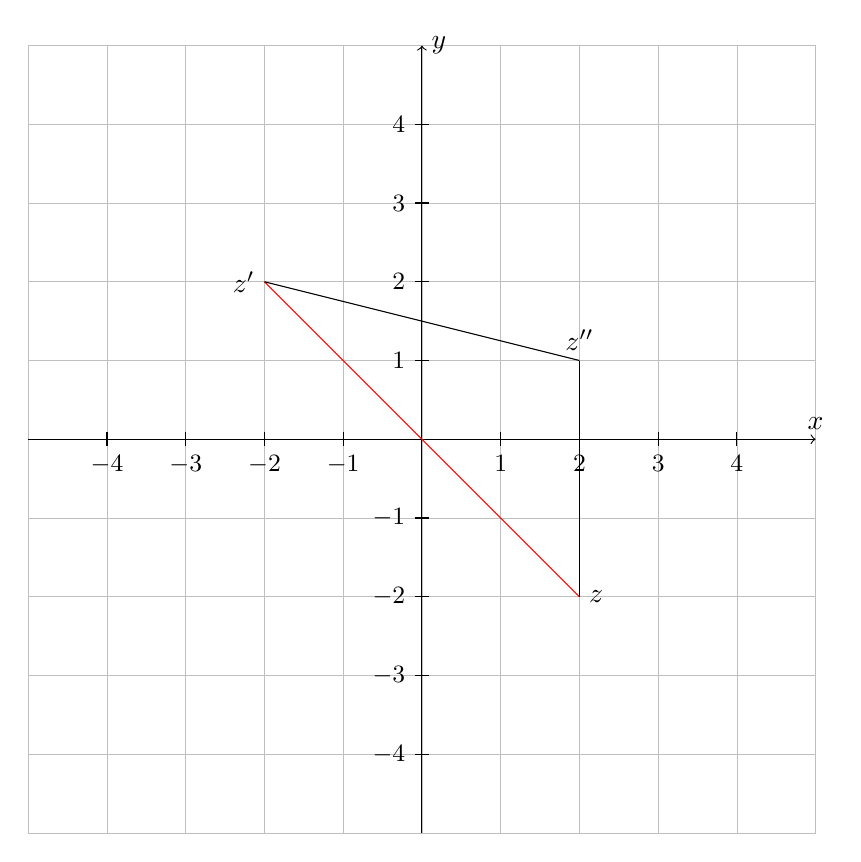
\begin{tikzpicture}
	\path [draw, help lines, opacity=.5]  (-5,-5) grid (5,5);
	\foreach \i in {1,...,4} \draw (\i,2.5pt) -- +(0,-5pt) node [anchor=north, font=\small] {$\i$} (-\i,2.5pt) -- +(0,-5pt) node [anchor=north, font=\small] {$-\i$} (2.5pt,\i) -- +(-5pt,0) node [anchor=east, font=\small] {$\i$} (2.5pt,-\i) -- +(-5pt,0) node [anchor=east, font=\small] {$-\i$};
	\draw [->] (-5,0) -- (5,0) node [anchor=south] {$x$};
	\draw [->] (0,-5) -- (0,5) node [anchor=west] {$y$};
	\draw [red,-] (-2,2) -- (2,-2) node [black, anchor=west] {$z$};
	\draw [-] (2,1) -- (-2,2) node [anchor=east] {$z'$};
	\draw [-] (2,-2) -- (2,1) node [anchor=south] {$z''$};
\end{tikzpicture}
